\documentclass{beamer}

\usepackage[english]{babel}
\usepackage{amsmath}

\begin{document}

\title{Smoothing In Naive Bayes and Language Models}
\author{Cheng Bing}
\date{\today}
\frame{\titlepage}

\begin{frame}
    \frametitle{Outline}
    \tableofcontents
\end{frame}

\section{Motivation}
\begin{frame}
\frametitle{Motivations of Smoothing}
MLE (Maximum Likelihood Estimation) works fine for items with large frequency. \\
For low frequency items, MLE suffers from:
\begin{itemize}
  \item Low Frequency Item Problem.
  \item Zero Count Problem.
\end{itemize}
\end{frame}

\begin{frame}
\frametitle{Motivations of Smoothing}
\begin{center}
Graphical Illustration.
\begin{figure}
  % Requires \usepackage{graphicx}
  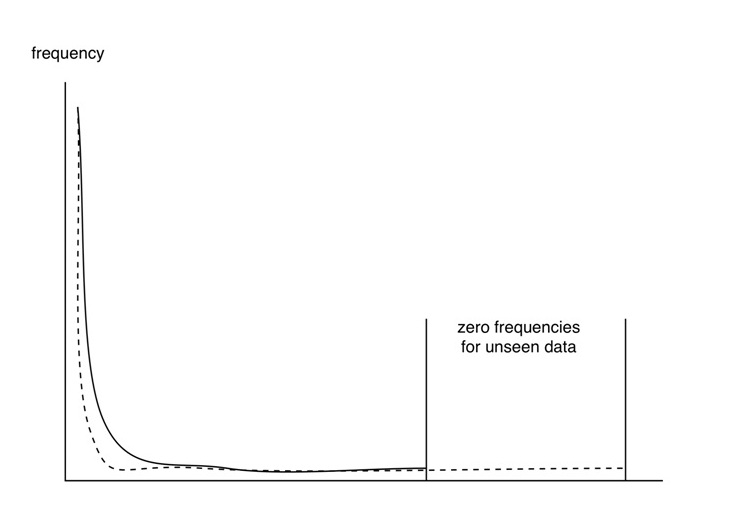
\includegraphics[width=8cm]{fig/smoothing-dis.jpg}\\
  \label{smoothing-dis}
\end{figure}
\end{center}
\end{frame}

\section{Naive Bayes Review}
\begin{frame}
\frametitle{Naive Bayes Review}
Suppose $c$ is class, $d$ is the document to be classified.
\begin{eqnarray*}
    P_{\theta_{c}}(d) &=& \frac{P_{\theta_{c}}(d)P(c)}{P(d)} \\
     & \varpropto & P_{\theta_{c}}(d)P(c) \\
     & \varpropto & P(c)\prod_{w \in d}P_{\theta_{c}}(w)
\end{eqnarray*}
$\theta_{c}$ comes from MLE (Maximum Likelihood Estimation) of word $w$ in collection $T_{c}$
\begin{equation*}
    P_{\theta_{c}}(w) = \frac{c(w)}{|T_{c}|}
\end{equation*}
\end{frame}

\section{Introduction to Language Model}
\begin{frame}
\frametitle{Introduction to Language Model}
LM (Language Model) is usually used to predict the next word in a speech sequence.\\
\textit{n-gram} LM: the choice of current word depends on the previous $n-1$ words.
\begin{equation*}
    P(w_{i} | w_{i-1}, w_{i-2} \cdots w_{0}) = P(w_{i} | w_{i-1}, w_{i-2} \cdots w_{i-n+1})
\end{equation*}

An example on how to estimate $P(w_{3}, w_{2}, w_{1})$
\begin{itemize}
  \item Unigram LM (Bag of Words)\\
        $P(w_{3}, w_{2}, w_{1})= P(w_{3})P(w_{2})P(w_{1})$
  \item Bigram LM\\
        $P(w_{3}, w_{2}, w_{1})=P(w_{3}|w_{2})P(w_{2}|w_{1})P(w_{1})$
\end{itemize}

\end{frame}

\section{Selected Smoothing Methods}
\begin{frame}
\frametitle{Selected Smoothing Methods}
\begin{itemize}
  \item Laplace Smoothing (Add One Smoothing)
  \item Jelinek-Mercer smoothing
  \item Dirichlet Priors
  \item Absolute discounting
  \item Katz smoothing
  \item Good-Turing Smoothing
\end{itemize}
\end{frame}

\section{Experimental Results of Laplace and Good-Turing Smoothing Applied to Naive Bayes}
\begin{frame}
\end{frame}

\end{document}